\section{整型数据}


\begin{frame}\ft{整数的存储方式}
数据都是以二进制的形式存储。\vspace{0.1in}

整数以补码的方式存储。\vspace{0.1in}

\begin{enumerate}
\item
正数的补码是其本身\\[0.1in]
\item 
负数的补码:将其绝对值的二进制形式按位取反再加1。
\end{enumerate}
\end{frame}
%
\begin{frame}\ft{整数的存储方式}

  \begin{figure}
    \centering
    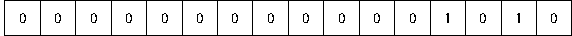
\includegraphics[]{ch03/images/positive_storage}
    \caption{正数10的存储方式}
  \end{figure}
%   
  \begin{figure}
    \centering
    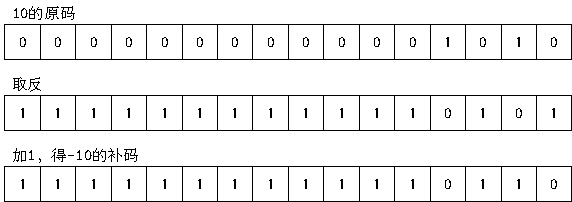
\includegraphics[]{ch03/images/negative_storage}
    \caption{负数-10的存储方式}
  \end{figure}
\end{frame}
% %
\begin{frame}[fragile]\ft{\lstinline|int|型}
\lstinline|int|型表示有符号整数,其取值范围依赖于系统,可通过以下代码查看。

\lstinputlisting[language=C,numbers=left,frame=single]{ch03/code/int_max_min.c}
\end{frame}

\begin{frame}[fragile]\ft{\lstinline|int|型}
\begin{lstlisting}
$ gcc int_max_min.c
$ ./a.out
range of int is -2147483648 ~ 2147483647
sizeof int = 4 bytes
\end{lstlisting}
\end{frame}
%
\begin{frame}[fragile]\ft{\lstinline|int|变量的声明}
\lstinline|int|用于声明基本的整型变量:
\begin{lstlisting}
int var;
int var1, var2;
\end{lstlisting}  \vspace{0.05in}

要声明多个变量,\vspace{0.05in}
\begin{itemize}
\item 可逐个声明每个变量;\\[0.1in]
\item 也可在\lstinline|int|后跟一个变量名列表,各变量之间用逗号隔开。
\end{itemize}

\end{frame}
%
\begin{frame}[fragile]\ft{\lstinline|int|变量的赋值}
赋值有三种方式:\vspace{0.05in}

\begin{enumerate}
\item 先声明,后赋值
\begin{lstlisting}[language=c]
int n;
n = 1;
\end{lstlisting}
\item 先声明,后通过\lstinline|scanf()|赋值
\begin{lstlisting}[language=c]
int n;
scanf("%d", &n);
\end{lstlisting} 
\item 初始化变量
\begin{lstlisting}[language=c]
int n = 1;
\end{lstlisting} 
\end{enumerate}
\end{frame}
% %
% %
\begin{frame}[fragile]\ft{\lstinline|int|变量的初始化}
初始化变量就是为变量赋一个初始值。
\begin{lstlisting}[language=c]
int a = 1;
int b = 2, c = 3;
int d, e = 4;  // valid, but not good
\end{lstlisting}
请避免在一个声明语句中同时出现初始化和未初始化的变量。
\end{frame}
%
\begin{frame}[fragile]\ft{\lstinline|int|变量的初始化}
  声明语句为变量创建、标定存储空间并为其指定初始值。 \pause 

  \begin{figure}
    \centering
    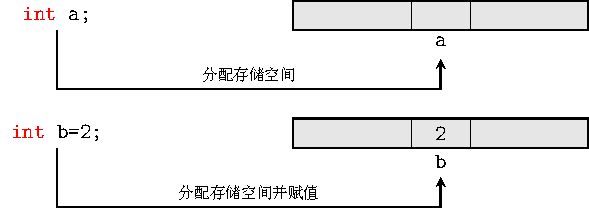
\includegraphics[]{ch03/images/var_def_and_init}
    \caption{定义和初始化变量}
  \end{figure}


\end{frame}
% 
%
\begin{frame}[fragile]\ft{\lstinline|int|值的打印}

\lstinputlisting[language=c,frame=single,numbers=left]{
ch03/code/print1.c
} 
\end{frame}
% 
%
\begin{frame}[fragile]\ft{\lstinline|int|值的打印}
\begin{lstlisting}[language=c]
$ gcc print1.c
$ ./a.out
Doing it right: 10 - 2 = 8
Doing it wrong: 10 - 73832 = 771
\end{lstlisting}
\end{frame}
% %
% %
\begin{frame}[fragile]\ft{\lstinline|int|值的打印}
在第二次调用print函数时,程序使用a为第一个\lstinline|%d|提供打印值,然后用内存中的任意值为其余两个\lstinline|%d|提供打印值。\vspace{0.1in}

注意: 使用printf函数时,格式说明符的个数与要显示值的数目必须相同。
\end{frame}
%
%
\begin{frame}[fragile]\ft{八进制数和十六进制数的打印}
在C中,有专门的前缀指明进制。

\begin{itemize}
\item 前缀\lstinline|0x|或\lstinline|0X|表示十六进制数\\[0.1in]
\item[] \lstinline|16|的十六进制表示为\lstinline|0x10|或\lstinline|0X10|。\\[0.2in]
\item 前缀\lstinline|0|表示八进制数\\[0.1in]
\item[] \lstinline|16|的八进制表示为\lstinline|020|。
\end{itemize}
\end{frame}

\begin{frame}[fragile]\ft{打印八进制数和十六进制数}
\lstinputlisting[language=c,frame=single,numbers=left]{
ch03/code/bases.c
}
\pause 
\begin{lstlisting}[language=c]
$ gcc bases.c
$ ./a.out
dec = 100; octal = 144; hex = 64
dec = 100; octal = 0144; hex = 0x64
\end{lstlisting}
\end{frame}
% %
\begin{frame}[fragile]\ft{八进制数和十六进制数的打印}
  \begin{table}
    \centering
    \begin{tabular}{c|c|c} \hline
      进制&格式说明符&格式说明符(显示前缀)\\\hline
      十进制& \lstinline|%d| & \\
      八进制& \lstinline|%o| & \lstinline|%#o|\\
      十六进制& \lstinline|%x|或\lstinline|%X|  & \lstinline|%#x|或\lstinline|%#X|\\\hline
    \end{tabular}
  \end{table}
\end{frame}
% %
\begin{frame}[fragile]\ft{其他整数类型}
C提供3个附属关键字修饰\lstinline|int|: \lstinline|short|、\lstinline|long|和\lstinline|unsigned|。
\end{frame}
% %
\begin{frame}[fragile]\ft{其他整数类型}
  \begin{table}
    \centering
    \begin{tabular}{p{2.8cm}|p{4.4cm}|p{3cm}} \hline
      类型&含义&占位符\\\hline
      \lstinline|short (int)|&   用于仅需小数值的场合 &  \lstinline|%hd, %ho, %hx|\\[0.1in]\hline
      \lstinline|long (int)| &   用于使用大数值的场合 &  \lstinline|%ld, %lo, %lx|\\[0.1in]\hline
      \lstinline|long long (int)|& 用于使用更大数值的场合(C99标准)&  \lstinline|%lld, %llo, %llx|  \\
      \hline
    \end{tabular}
  \end{table}
\end{frame}

\begin{frame}[fragile]\ft{其他整数类型}
  \begin{table}
    \centering
    \begin{tabular}{p{2.8cm}|p{4.4cm}|p{3cm}} \hline
      类型&含义&占位符\\\hline
      \lstinline|unsigned (int)|&  用于只使用非负值的场合。16位的取值范围是0-65535。  & \lstinline|%u|\\[0.1in]\hline
      \lstinline|unsigned long (int)| &   (C90标准)& \lstinline|%lu| \\[0.1in]\hline
      \lstinline|unsigned long long (int)|   & (C99标准) &\lstinline|%llu|\\
      \hline
    \end{tabular}
  \end{table}
\end{frame}
%
\begin{frame}[fragile]\ft{其他整数类型}
  关键字\lstinline|signed|可以和任何有符号类型一起使用,使数据类型更加明确。
  如\lstinline|short|、\lstinline|short int|、\lstinline|signed short|和\lstinline|signed short int|表示同一种类型。
\end{frame}
%
\begin{frame}[fragile]\ft{为什么会出现多种整数类型?}
C仅保证\lstinline|short|类型不会比\lstinline|int|类型长,\lstinline|long|类型不会比\lstinline|int|类型短,其目的是为了适应不同的机器。\vspace{0.05in}

\begin{itemize}
\item 有些CPU的自然字大小,若认为没有表示更大数的需要,会将\lstinline|long|类型和\lstinline|int|类型定义相同的长度。\\[0.1in]
\item 很多场合不要用到太大的整数,于是创建了更节省空间的\lstinline|short|类型。
\end{itemize}
\end{frame}

\begin{frame}[fragile]\ft{整数的上溢}
\begin{wenti}
若整数太大,超出整数类型的范围会发生什么?
\end{wenti}
\end{frame}

\begin{frame}[fragile]\ft{整数的上溢}
\lstinputlisting[language=c,frame=single,numbers=left]{
ch03/code/IntOverflow.c
}
\end{frame}
%
\begin{frame}[fragile]\ft{整数的上溢}

\begin{lstlisting}[language=c]
$ gcc IntOverflow.c
$ ./a.out
i = 2147483647, i+1 = -2147483648, i+2 = -2147483647
j = 4294967295, j+1 = 0, j+2 = 1
\end{lstlisting}
\end{frame}
%
\begin{frame}[fragile]\ft{整数的上溢}

当达到最大值时,将溢出到起始点。\vspace{0.05in}
\begin{itemize}
\item 对于\lstinline|unsigned int|类型,起始点是0;\\[0.1in]
\item 对于\lstinline|int|类型,起始点为-2147483648。
\end{itemize}

\vspace{0.1in}
 注意: 当整数溢出时,编译器不会给出任何提示,故编程时必须谨慎对待此类问题。 

\end{frame}
